\section{Requirements Captured}
The following are requirement divided into functional and non-functional requirement which where collected after consulting with the client.
\subsection*{Functionality requirements}
The list of the requirements for the application where as follows:
\newline\textbf{Functional Requirements}
\begin{itemize}
	\item Rendering of the map on the user screen
	\item Have signal strength indicators on the map. These should be updated on a real-time basis.
	\item Save signal strength on the database for a specific location.
	\item Zoom in and zoom out of the campus map
\end{itemize}
\textbf{Non-Functional Requirements}
\begin{itemize}
	\item Real-time receiving of data being updated in the database.
	\item Speed up on the rendering of the areas and their strengths on the map.
\end{itemize}



The next section deals with the analysis of your system. Cover the
functional, non-functional and usability requirements. This is where
you present your use case narratives and diagrams. 

Discuss the major analysis artefacts that you produced. We will expect
you to produce at least one overall description of the architecture
used in your system as a diagram, either here or below (see Section
\ref{ss:design-overview}). You may also want to include an analysis
class hierarchy diagram.

\subsection*{Use case}
Below is a use case diagram to show the different operation that can be done on the system and the actors who are responsible for performing these actions. Firstly, there is a need to discuss the different users of the systems and the different systems that are used by our system. These make up the actors involved in the system. The different actors and their level of interaction with the application are listed below:
\newline\textbf{Primary Actor}
\begin{itemize}
	\item User
	\item ICTS (extending User)
	\item Phone
\end{itemize}
\textbf{Secondary users}
\begin{itemize}
	\item Server (where the application data )
	\item User (for some instances.)
\end{itemize}
\pagebreak
\begin{figure}
	\centering
	\includegraphics[width=0.7\linewidth]{"images/Use Case"}
	\caption{Showing the use case diagram of the Wi-Fi Mapper}
	\label{fig:use-case}
\end{figure}
The main use case for the system is update WLAN Zone information as it is the spawns many more functions that influence the user's view of the menu. The detailed flow of events for updating information of a particular zone are shown by the use case narrative below:
\newline
\begin{tabular}{|p{0.21\textwidth}|p{0.3\textwidth}|p{0.24\textwidth}|p{0.25\textwidth}|}
	\hline
	\textbf{Use Case:} & Update WLAN Zone & \textbf{ID:} 007 & \textbf{Level:} High
	\\\hline
	\textbf{Actors:} & \multicolumn{3}{|l|}{Users, ICTS, Wi-Fi Mapper Server} \\\hline
	\multirow{2}{0.2\textwidth}{\textbf{Stakeholders and Interests}} &
	\multicolumn{3}{|p{0.79\textwidth}|}{
		Josiah Chavula -The owner of the product,
	} \\
	& \multicolumn{3}{|p{0.79\textwidth}|}{
		ICTS - they use the information provided by the system.
	} \\\hline
	\textbf{Brief Description:} & \multicolumn{3}{|p{0.79\textwidth}|}{
	A user who is using the app opens the application to get the different eduroam strength signals. The system gives user the data for the whole UCT upper campus map. If location permissions are granted the user is then also able to send their data to the server and get the map zoomed in to give them strength signals on a few meters radius around them.} \\\hline
	\multirow{2}{0.2\textwidth}{\textbf{Preconditions:}}
	& \multicolumn{3}{|p{0.79\textwidth}|}{
		User connected to eduroam.} \\
	& \multicolumn{3}{|p{0.79\textwidth}|}{
		User is at the locations that are supported by the application.} \\\hline
	\multirow{3}{0.2\textwidth}{\textbf{Post Conditions:}}
	& \multicolumn{3}{|p{0.79\textwidth}|}{Data is updated at the server.} \\
	& \multicolumn{3}{|p{0.79\textwidth}|}{User has a data showing different signal strengths across the UCT Campus.}  \\\hline
	\multirow{1}{0.2\textwidth}{\textbf{Related Use Cases:}}
	& \multicolumn{3}{|p{0.79\textwidth}|}{includes: Get user permissions} \\\hline
\end{tabular}

\begin{longtable}{|p{0.5\textwidth}|p{0.5\textwidth}|}\hline
	\multicolumn{2}{|p{1.095\textwidth}|}{\textbf{Typical Course of Events}} \\\hline
	\textbf{Actor Action} & \textbf{System Response} \\\hline
	\begin{enumerate}[series=typical]
		\item Phone Queries the database for data for the supported areas and return to user. 
	\end{enumerate} &
	\begin{enumerate}[resume=typical]
		\item Queries the database for data for the supported areas and return to user
		\item Request user to give location permissions
	\end{enumerate}
	\\\hline
	\begin{enumerate}[resume=typical]
		\item Grants the system permission to use Location services
	\end{enumerate} &
	\begin{enumerate}[resume=typical]
		\item Get the current user location
		\item Get the signal Strength of the users Wi-Fi
		\item Set up Location Change listener
	\end{enumerate}
	\\\hline
	\begin{enumerate}[resume=typical]
		\item Continuously send the system data from where they are located.
	\end{enumerate}
	&
	\begin{enumerate}[resume=typical]
		\item Constantly accepts data from the users 
		\item Save the data
		\item Use aggregate data from the users to calculate average strength signals for different locations.
	\end{enumerate} \\\hline
	\begin{enumerate}[resume=typical]
		\item User changes zoom level
	\end{enumerate}
	& 
	\begin{enumerate}[resume=typical]
		\item System changes the focus level for the specific area.
	\end{enumerate}
	\\\hline
\end{longtable}

\begin{longtable}{|p{0.5\textwidth}|p{0.5\textwidth}|}\hline
	\multicolumn{2}{|p{1.095\textwidth}|}{\textbf{Alternative Courses of Events}} \\\hline
	\textbf{Actor Action} & \textbf{System Response} \\\hline
	\begin{enumerate}
		\setcounter{enumi}{3}
		\item 
		\begin{enumerate}[series=abnormal0]
			\item Refuse to give the system location permissions
		\end{enumerate}
	\end{enumerate}
	&
	\begin{enumerate}[series=abnormal0]
		\setcounter{enumi}{4}
		\item
		\begin{enumerate}
			\item Continue showing the user the upper campus map without giving them information about where they are. 
		\end{enumerate}
	\end{enumerate} \\\hline
	\begin{enumerate}
		\setcounter{enumi}{7}
		\item 
		\begin{enumerate}[series=abnormal1]
			\item User loses signal to send data to the server
		\end{enumerate}
	\end{enumerate}
	&
	\begin{enumerate}
		\setcounter{enumi}{8}
		\item 
		\begin{enumerate}
			\item User loses signal to send data to the server
			\item System notifies user that disconnection occurred
		\end{enumerate}
	\end{enumerate} \\\hline
\end{longtable}

\subsection*{Design Overview}
\label{ss:design-overview}
\paragraph{}This Section gives an overview of the system which entails showing how the system interacts with other systems in delivery of functionality to the user and introduce the basic functionality expected from the System,It will also describe what type of stakeholders will interact with the system and what functionality each should expect,finally explain the assumptions and constraints for the system 

\paragraph{}They are mainly Two ways users can interact with the System that is through a mobile Application(Android Only) and Web Application.

\paragraph{}Mobile Application will need to communicate with the phone's GPS system so as to obtain a user's Location.The functionality provided by GPS is crucial as it pinpoints exactly which WLAN Zone data is collected and ensures accurate aggregate Data is displayed on each WLAN zone.

\paragraph{}Wifi Manager will also be needed by the mobile application so as to obtain Wifi Strength of the router to which the mobile phone is connected to a certain point in time,as both the Wifi Strength and Location to which this data is obtained are the main pieces of information driving the System.

\paragraph{}Since this is a data-centric Application,that means data needs to be stored in a database,both Web Application and Mobile Application will communicate with the database but in slightly different ways.Mobile Application will both query and send data to and from the database while
the web Application will be restricted to just querying data from the database for displaying purposes.

\paragraph{}Query Manager is used by both Mobile so as to validate the data collected corresponds to a WLAN zone or else its not written to the database and handles requests of data from both web and Mobile Application to obtain data to display.

\paragraph{}Both Mobile and Web Application use the Mapping System so as to display a Map to the user which includes data collected from the users stored in the database aggregated into different WLAN zones so as to provide appropriate information to the user.

\paragraph{}Cluster System is required by the Mapping System so as to cluster Data points collected which are very close to each other so as to prevent clutter on the Map which is undesirable to the user(Clustering occurs only at high zoom level).  

\paragraph{}Reporting system is used by the Web Client to generate a report which will provide useful information based on the collected data stored in the database.   
 
\begin{figure}
	\centering
	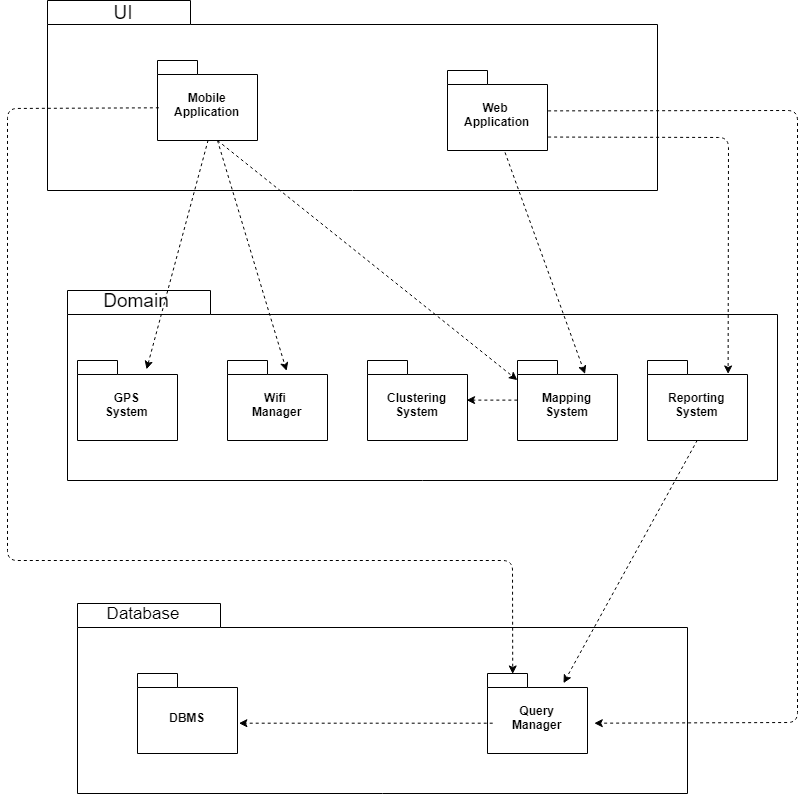
\includegraphics[width=0.7\linewidth]{images/Architecture}
	\caption{Architecture Diagram}
	\label{fig:architecture}
\end{figure}

